\documentclass{beamer}
\usefonttheme[onlymath]{serif}
\usepackage[T1]{fontenc}
\usepackage[utf8]{inputenc}
\usepackage[english, icelandic]{babel}
\usepackage{amsmath}
\usepackage{amssymb}
\usepackage{amsthm}
\usepackage{gensymb}
\usepackage{parskip}
\usepackage{mathtools}
\usepackage{listings}
\usepackage{hyperref}
\usepackage{graphicx}
\usepackage{color}
\usepackage{enumerate}
\usepackage{tikz}
\usetikzlibrary{calc}
\usetikzlibrary{positioning}
\usetikzlibrary{angles}
\usetikzlibrary{shapes}
\usetikzlibrary{arrows}
\usepackage{verbatim}
\usepackage{multicol}
\usepackage{array}
\usepackage{minted}
\parskip 0pt

\DeclareMathOperator{\lcm}{lcm}
\newcommand\floor[1]{\left\lfloor#1\right\rfloor}
\newcommand\ceil[1]{\left\lceil#1\right\rceil}
\newcommand\abs[1]{\left|#1\right|}
\newcommand\p[1]{\left(#1\right)}
\newcommand\sqp[1]{\left[#1\right]}
\newcommand\cp[1]{\left\{#1\right\}}
\newcommand\norm[1]{\left\lVert#1\right\rVert}
\renewcommand\Im{\operatorname{Im}}
\renewcommand\Re{\operatorname{Re}}

\usetheme{metropolis}
\definecolor{dark yellow}{rgb} {0.6,0.6,0.0}
\definecolor{dark green}{rgb} {0.0,0.6,0.0}

\graphicspath{{myndir/}}

\tikzstyle{vertex}=[circle,fill=black!50,minimum size=15pt,inner sep=0pt, font=\small]
\tikzstyle{selected vertex} = [vertex, fill=red!24]
\tikzstyle{edge} = [draw,thick,-]
\tikzstyle{dedge} = [draw,thick,->]
\tikzstyle{weight} = [font=\scriptsize,pos=0.5]
\tikzstyle{selected edge} = [draw,line width=2pt,-,red!50]
\tikzstyle{ignored edge} = [draw,line width=5pt,-,black!20]

\tikzset{
  treenode/.style = {align=center, inner sep=0pt, text centered,
    font=\sffamily},
  vertex/.style = {treenode, circle, black, font=\sffamily\bfseries\tiny, draw=black, text width=1.8em},% arbre rouge noir, noeud noir
  rvertex/.style = {treenode, circle, black, font=\sffamily\bfseries\tiny, draw=red, text width=1.8em},% arbre rouge noir, noeud noir
}

\title{Data Structures}
\author{Arnar Bjarni Arnarson}
\institute{\href{http://ru.is/td}{School of Computer Science} \\[2pt] \href{http://ru.is}{Reykjavík University}}
\titlegraphic{\hfill
\includegraphics[height=0.6cm]{../../shared/kattis}}

\begin{document}
\maketitle

\begin{frame}[plain]{Today's material}
    \begin{itemize}
        \item Built-in data structures and their applications
        \item Augmenting a data structure        
        \item Union-Find
        \item Precomputations like prefix sums
        \item Square root decomposition
        \item Segment trees
        \item Sparse tables
    \end{itemize}
\end{frame}

\begin{frame}{Applications of Arrays and Linked Lists}
    \vspace{40pt}
    \begin{itemize}
        \item<1-> Too many to list, more so for arrays
        \item<2-> Most problems require storing data, usually in an array
        \item<3-> On modern machines, arrays are almost always a better choice than a linked list
        \item<4-> There are however a few cases where linked lists are better
    \end{itemize}
\end{frame}

\begin{frame}{Example problem: Broken Keyboard}
    \begin{itemize}
        \item http://uva.onlinejudge.org/external/119/11988.html
    \end{itemize}
\end{frame}

\begin{frame}{Applications of Stacks}
    \begin{itemize}
        \item<1-> Processing events in a last-in first-out order
        \item<2-> Simulating recursion
        \item<3-> Depth-first search in a graph
        \item<4-> Reverse a sequence
        \item<5-> Matching brackets
        \item<6-> And a lot more
    \end{itemize}
\end{frame}

% \begin{frame}{Example problem: Backspace}
%     \begin{itemize}
%         \item https://open.kattis.com/problems/backspace
%     \end{itemize}
% \end{frame}

\begin{frame}{Applications of Queues}
    \begin{itemize}
        \item<1-> Processing events in a first-in first-out order
        \item<2-> Breadth-first search in a graph
        \item<3-> Scheduling tasks and distributing tasks
        \item<4-> Also used by network protocols to manage messages
        \item<5-> Used for a lot of OS and hardware operations
        \item<6-> And a lot more
    \end{itemize}
\end{frame}

\begin{frame}{Applications of Priority Queues}
    \begin{itemize}
        \item<1-> Processing events in order of priority
        \item<2-> Finding a shortest path in a graph
        \item<3-> Some greedy algorithms
        \item<4-> And a lot more
    \end{itemize}
\end{frame}

\begin{frame}{Applications of Sets}
    \begin{itemize}
        \item<1-> Keep track of distinct items
        \item<2-> Have we seen an item before?
        \item<3-> If implemented as a binary search tree:
        \begin{itemize}
            \item<4-> Find the successor/predecessor of an element
            \item<5-> Count how many elements are less than a given element
            \item<6-> Count how many elements are between two given elements
            \item<7-> Find the $k$th largest element
        \end{itemize}
        \item<8-> And a lot more
    \end{itemize}
\end{frame}

\begin{frame}{Applications of Maps}
    \begin{itemize}
        \item<1-> Associating a value with a key
        \item<2-> As a frequency table
        \item<3-> As a memory when doing Dynamic Programming
        \item<4-> And a lot more
    \end{itemize}
\end{frame}

\begin{frame}{Augmenting Data Structures}
    \begin{itemize}
        \item<1-> Sometimes we can store extra information in our data structures to gain more functionality
        \item<2-> Usually we can't do this to data structures in the standard library
        \item<3-> Need our own implementation that we can customize
        \item<4-> Example: Augmenting binary search trees
    \end{itemize}
\end{frame}

\begin{frame}[fragile]{Augmenting Binary Search Trees}
    \begin{columns}[T]
        \begin{column}{.45\textwidth}
            \vspace{20pt}

            \begin{itemize}
                \item We have a binary search tree and want to efficiently:
                    \begin{itemize}
                        \item Count number of elements $<x$
                        \item Find the $k$th smallest element
                    \end{itemize}

                \item Naive method is to go through all vertices, but that is slow: $O(n)$
            \end{itemize}
        \end{column}%
        \hfill%
        \begin{column}{.55\textwidth}
            \begin{figure}

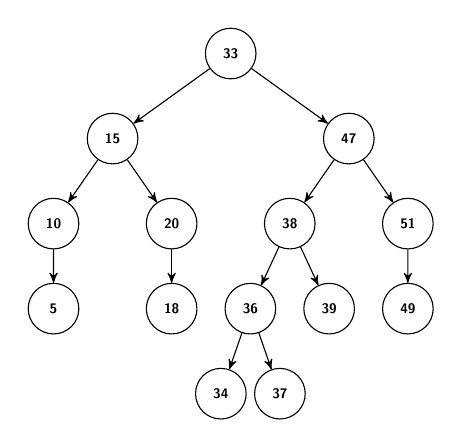
\begin{tikzpicture}[->,>=stealth',level/.style={sibling distance = 5cm/#1,
  level distance = 1.8cm},scale=0.6] 
\node [vertex] {33}
    child{ node [vertex] {15}
            child{ node [vertex] {10} 
            	child{ node [vertex] {5} } %for a named pointer
                % child{ node [vertex] {}}
            }
            child{ node [vertex] {20}
							child{ node [vertex] {18}}
							% child{ node [vertex] {}}
            }                            
    }
    child{ node [vertex] {47}
            child{ node [vertex] {38} 
							child{ node [vertex] {36}
                                child { node [vertex] {34} }
                                child { node [vertex] {37} }
                            }
							child{ node [vertex] {39}}
            }
            child{ node [vertex] {51}
							child{ node [vertex] {49}}
							% child{ node [vertex] {}}
            }
		}
; 
\end{tikzpicture}
            \end{figure}
        \end{column}%
    \end{columns}
\end{frame}

\begin{frame}[fragile]{Augmenting Binary Search Trees}

    \begin{columns}[T]
        \begin{column}{.45\textwidth}
            \vspace{20pt}

            \begin{itemize}
                \item Idea: In each vertex store the size of the subtree
                \item This information can be maintained when we insert/delete elements without increasing time complexity
            \end{itemize}
        \end{column}%
        \hfill%
        \begin{column}{.55\textwidth}
            \begin{figure}

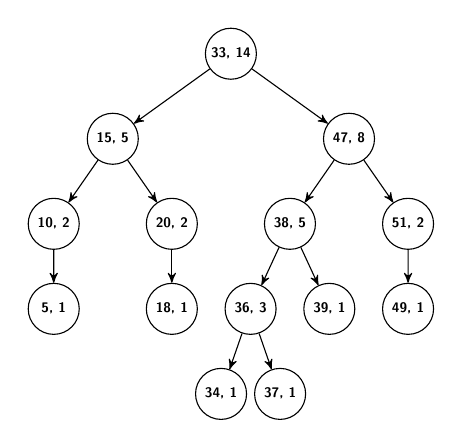
\begin{tikzpicture}[->,>=stealth',level/.style={sibling distance = 5cm/#1,
  level distance = 1.8cm},scale=0.6] 
\node [vertex] {33, 14}
    child{ node [vertex] {15, 5}
            child{ node [vertex] {10, 2} 
            	child{ node [vertex] {5, 1} } %for a named pointer
                % child{ node [vertex] {}}
            }
            child{ node [vertex] {20, 2}
							child{ node [vertex] {18, 1}}
							% child{ node [vertex] {}}
            }                            
    }
    child{ node [vertex] {47, 8}
            child{ node [vertex] {38, 5} 
							child{ node [vertex] {36, 3}
                                child { node [vertex] {34, 1} }
                                child { node [vertex] {37, 1} }
                            }
							child{ node [vertex] {39, 1}}
            }
            child{ node [vertex] {51, 2}
							child{ node [vertex] {49, 1}}
							% child{ node [vertex] {}}
            }
		}
; 
\end{tikzpicture}
            \end{figure}
        \end{column}%
    \end{columns}
\end{frame}

\begin{frame}[fragile]{Augmenting Binary Search Trees}

    \begin{columns}[T]
        \begin{column}{.45\textwidth}
            \begin{itemize}
                \item Count number of elements $<38$
                    \begin{itemize}
                        \item Search for $38$ in the tree
                        \item Count the vertices that we pass by that are less than $x$
                        \item When we are at a vertex where we should go right, get the size of the left subtree and add it to our count
                    \end{itemize}
            \end{itemize}
        \end{column}%
        \hfill%
        \begin{column}{.55\textwidth}
            \begin{figure}
                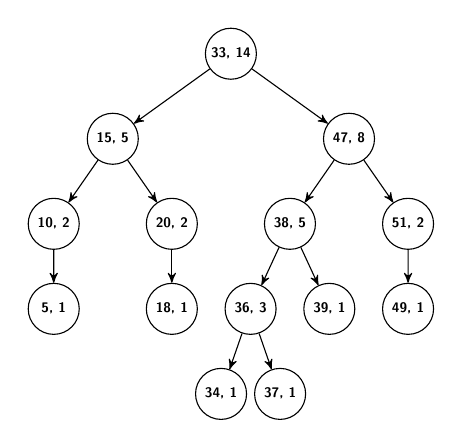
\begin{tikzpicture}[->,>=stealth',level/.style={sibling distance = 5cm/#1,
  level distance = 1.8cm},scale=0.6] 
\node [vertex] {33, 14}
    child{ node [vertex] {15, 5}
            child{ node [vertex] {10, 2} 
            	child{ node [vertex] {5, 1} } %for a named pointer
                % child{ node [vertex] {}}
            }
            child{ node [vertex] {20, 2}
							child{ node [vertex] {18, 1}}
							% child{ node [vertex] {}}
            }                            
    }
    child{ node [vertex] {47, 8}
            child{ node [vertex] {38, 5} 
							child{ node [vertex] {36, 3}
                                child { node [vertex] {34, 1} }
                                child { node [vertex] {37, 1} }
                            }
							child{ node [vertex] {39, 1}}
            }
            child{ node [vertex] {51, 2}
							child{ node [vertex] {49, 1}}
							% child{ node [vertex] {}}
            }
		}
; 
\end{tikzpicture}
            \end{figure}
        \end{column}%
    \end{columns}
\end{frame}
\begin{frame}[fragile]{Augmenting Binary Search Trees}

    \begin{columns}[T]
        \begin{column}{.45\textwidth}
            \begin{itemize}
                \item Count number of elements $<38$
                    \begin{itemize}
                        \item Search for $38$ in the tree
                        \item Count the vertices that we pass by that are less than $x$
                        \item When we are at a vertex where we should go right, get the size of the left subtree and add it to our count
                    \end{itemize}
                \vspace{2pt}
                \item Time complexity $O(\log n)$
            \end{itemize}
        \end{column}%
        \hfill%
        \begin{column}{.55\textwidth}
            \begin{figure}
                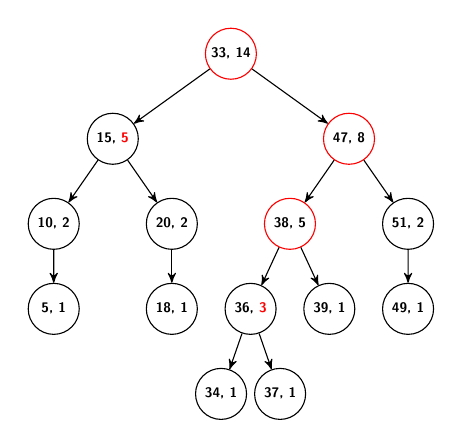
\begin{tikzpicture}[->,>=stealth',level/.style={sibling distance = 5cm/#1,
  level distance = 1.8cm},scale=0.6] 
\node [rvertex] {33, 14}
    child{ node [vertex] {15, {\color{red}5}}
            child{ node [vertex] {10, 2} 
            	child{ node [vertex] {5, 1} } %for a named pointer
                % child{ node [vertex] {}}
            }
            child{ node [vertex] {20, 2}
							child{ node [vertex] {18, 1}}
							% child{ node [vertex] {}}
            }                            
    }
    child{ node [rvertex] {47, 8}
            child{ node [rvertex] {38, 5} 
                            child{ node [vertex] {36, {\color{red}3}}
                                child { node [vertex] {34, 1} }
                                child { node [vertex] {37, 1} }
                            }
							child{ node [vertex] {39, 1}}
            }
            child{ node [vertex] {51, 2}
							child{ node [vertex] {49, 1}}
							% child{ node [vertex] {}}
            }
		}
; 
\end{tikzpicture}
            \end{figure}
        \end{column}%
    \end{columns}
\end{frame}

% \begin{frame}[fragile]{Augmenting Binary Search Trees}
%
%     \begin{columns}[T]
%         \begin{column}{.45\textwidth}
%             \begin{itemize}
%                 \item Count number of elements $<38$
%                     \begin{itemize}
%                         \item Search for $38$ in the tree
%                         \item Count the vertices that we pass by that are less than $x$
%                         \item When we are at a vertex where we should go right, get the size of the left subtree and add it to our count
%                     \end{itemize}
%                 % \vspace{2pt}
%                 % \item Time complexity $O(\log n)$
%             \end{itemize}
%         \end{column}%
%         \hfill%
%         \begin{column}{.55\textwidth}
%             \begin{figure}
%
% \begin{tikzpicture}[->,>=stealth',level/.style={sibling distance = 5cm/#1,
%   level distance = 1.8cm},scale=0.6] 
% \node [rvertex] {33, 14}
%     child{ node [vertex] {15, {\color{red}5}}
%             child{ node [vertex] {10, 2} 
%             	child{ node [vertex] {5, 1} } %for a named pointer
%                 % child{ node [vertex] {}}
%             }
%             child{ node [vertex] {20, 2}
% 							child{ node [vertex] {18, 1}}
% 							% child{ node [vertex] {}}
%             }                            
%     }
%     child{ node [rvertex] {47, 8}
%             child{ node [rvertex] {38, 5} 
%                             child{ node [vertex] {36, {\color{red}3}}
%                                 child { node [vertex] {34, 1} }
%                                 child { node [vertex] {37, 1} }
%                             }
% 							child{ node [vertex] {39, 1}}
%             }
%             child{ node [vertex] {51, 2}
% 							child{ node [vertex] {49, 1}}
% 							% child{ node [vertex] {}}
%             }
% 		}
% ; 
% \end{tikzpicture}
%             \end{figure}
%         \end{column}%
%     \end{columns}
% \end{frame}

\begin{frame}[fragile]{Augmenting Binary Search Trees}

    \begin{columns}[T]
        \begin{column}{.45\textwidth}
            \begin{itemize}
                \item Find $k$th smallest element
                    \begin{itemize}
                        \item We're on a vertex whose left subtree is of size $m$
                        \item If $k = m+1$, we found it
                        \item If $k \leq m$, look for the $k$th smallest element in the left subtree
                        \item If $k > m+1$, look for the $k-m-1$st smallest element in the right subtree
                    \end{itemize}
                \vspace{2pt}
            \end{itemize}
        \end{column}%
        \hfill%
        \begin{column}{.55\textwidth}
            \begin{figure}
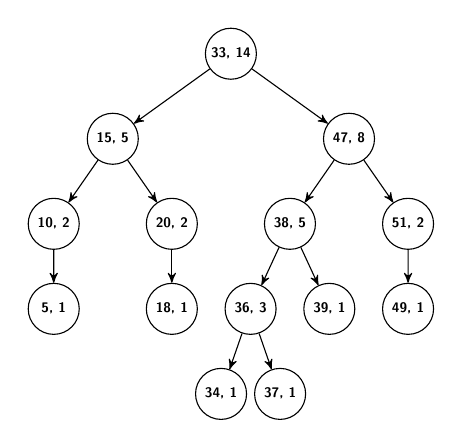
\begin{tikzpicture}[->,>=stealth',level/.style={sibling distance = 5cm/#1,
  level distance = 1.8cm},scale=0.6] 
\node [vertex] {33, 14}
    child{ node [vertex] {15, 5}
            child{ node [vertex] {10, 2} 
            	child{ node [vertex] {5, 1} } %for a named pointer
                % child{ node [vertex] {}}
            }
            child{ node [vertex] {20, 2}
							child{ node [vertex] {18, 1}}
							% child{ node [vertex] {}}
            }                            
    }
    child{ node [vertex] {47, 8}
            child{ node [vertex] {38, 5} 
                            child{ node [vertex] {36, 3}
                                child { node [vertex] {34, 1} }
                                child { node [vertex] {37, 1} }
                            }
							child{ node [vertex] {39, 1}}
            }
            child{ node [vertex] {51, 2}
							child{ node [vertex] {49, 1}}
							% child{ node [vertex] {}}
            }
		}
; 
\end{tikzpicture}
            \end{figure}
        \end{column}%
    \end{columns}
\end{frame}

\begin{frame}[fragile]{Augmenting Binary Search Trees}

    \begin{columns}[T]
        \begin{column}{.45\textwidth}
            \begin{itemize}
                \item Find $k$th smallest element
                    \begin{itemize}
                        \item We're on a vertex whose left subtree is of size $m$
                        \item If $k = m+1$, we found it
                        \item If $k \leq m$, look for the $k$th smallest element in the left subtree
                        \item If $k > m+1$, look for the $k-m-1$st smallest element in the right subtree
                    \end{itemize}
                \item Example: $k=11$
            \end{itemize}
        \end{column}%
        \hfill%
        \begin{column}{.55\textwidth}
            \begin{figure}
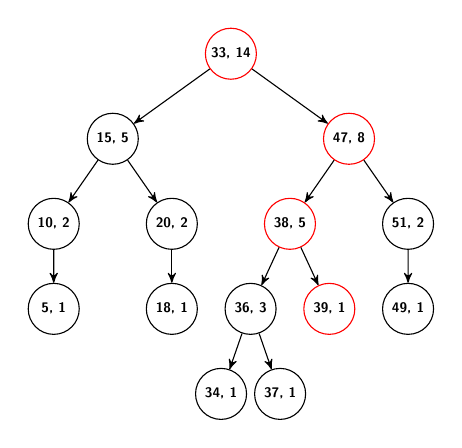
\begin{tikzpicture}[->,>=stealth',level/.style={sibling distance = 5cm/#1,
  level distance = 1.8cm},scale=0.6] 
\node [rvertex] {33, 14}
    child{ node [vertex] {15, 5}
            child{ node [vertex] {10, 2} 
            	child{ node [vertex] {5, 1} } %for a named pointer
                % child{ node [vertex] {}}
            }
            child{ node [vertex] {20, 2}
							child{ node [vertex] {18, 1}}
							% child{ node [vertex] {}}
            }                            
    }
    child{ node [rvertex] {47, 8}
            child{ node [rvertex] {38, 5} 
                            child{ node [vertex] {36, 3}
                                child { node [vertex] {34, 1} }
                                child { node [vertex] {37, 1} }
                            }
							child{ node [rvertex] {39, 1}}
            }
            child{ node [vertex] {51, 2}
							child{ node [vertex] {49, 1}}
							% child{ node [vertex] {}}
            }
		}
; 
\end{tikzpicture}
            \end{figure}
        \end{column}%
    \end{columns}
\end{frame}

\begin{frame}[plain]{Union-Find}
    \begin{itemize}
        \item<1-> We have $n$ items
        \item<2-> Maintains a collection of disjoint sets (or equivalently, an equivalence relation)
        \item<3-> Each of the $n$ items is in exactly one set
        \item<4-> We represent each set with one of its members, a representative element
        \item<5-> Supports two operations efficiently: \texttt{find(x)} and \texttt{union(x,y)}.
        \item<6-> Operation \texttt{find(x)} finds the representative of the set $x$ is in
        \item<7-> Operation \texttt{union(x, y)} unions the sets of which $x$ and $y$ are members.
    \end{itemize}
\end{frame}

\begin{frame}[plain]{Union-Find}
    \begin{itemize}
        \item<1-> It is generally initialized with all items being in their own set.
        \item<2-> So for $n = 5$ we start out with $\{\{1\},\{2\},\{3\},\{4\},\{5\}\}$.
        \item<3-> \texttt{join(1, 3)} then changes this to $\{\{1, 3\}, \{2\}, \{4\}, \{5\}\}$.
		\item<4-> \texttt{join(2, 5)} then results in $\{\{1, 3\}, \{2, 5\}, \{4\}\}$.
		\item<5-> \texttt{join(2, 4)} then results in $\{\{1, 3\}, \{2, 4, 5\}\}$.
		\item<6-> \texttt{join(1, 4)} finally results in $\{\{1, 2, 3, 4, 5\}\}$.
        \item<7-> At any given point $\texttt{find(x)}$ returns some value in the same set as $x$.
        \item<8-> The important bit is that \texttt{find(x)} returns the same value for all elements of the same set, the representative.
    \end{itemize}
\end{frame}

\begin{frame}[plain]{Union-Find}
    \begin{itemize}
        \item<1-> We can do this by maintaining an array of parents, letting the $i$-th value be the index of the parent of the $i$-th item.
        \item<2-> If a value has no parent, we can denote this somehow, make it its own parent, give it the value $-1$, exactly what we do is not important.
        \item<3-> To get the representative of $x$ we go to the parent of our current item (starting at $x$) until the item has no parent.
        \item<4-> Then to unite $x, y$ we simply make the representative of $x$ the parent of the representative of $y$.
    \end{itemize}
\end{frame}

\begin{frame}[plain,fragile]{Naïve Union-Find implementation}
    \begin{minted}{cpp}
struct union_find {
    vector<int> parent;
    union_find(int n) {
        parent = vector<int>(n);
        for(int i = 0; i < n; i++) {
            parent[i] = i;
        }
    }
    int find(int x) {
        return parent[x] == x ? x : find(parent[x]);
    }
    void unite(int x, int y) {
        parent[find(x)] = find(y);
    }
};
    \end{minted}
\end{frame}

\begin{frame}[plain]{Union-Find}
    \begin{itemize}
        \item<1-> The problem here is that for specific queries, the parent chains may end up being of length $\mathcal{O}(n)$, making each query linear.
        \item<2-> The key to making this more efficient is making those chains shorter.
        \item<3-> We do this by flattening the chain each time we query \texttt{find}, so the amortized complexity becomes good.
        \item<4-> The worst case is still $\mathcal{O}(n)$ but the amortized complexity is $\mathcal{O}(\alpha(n))$ which may as well be a constant, as it is $<5$ for $n$ equal to the number of atoms in the observable universe.
    \end{itemize}
\end{frame}

\begin{frame}[plain,fragile]{Path compressed Union-Find implementation}
    \begin{minted}{cpp}
struct union_find {
    vector<int> parent;
    union_find(int n) {
        parent = vector<int>(n);
        for (int i = 0; i < n; i++) {
            parent[i] = i;
        }
    }
    int find(int x) {
        if(parent[x] == x) return x;
        return parent[x] = find(parent[x]);
    }
    void unite(int x, int y) {
        parent[find(x)] = find(y);
    }
};
    \end{minted}
\end{frame}

\begin{frame}[plain]{Union-Find applications}
    \vspace{30pt}
    \begin{itemize}
        \item<1-> Union-Find maintains a collection of disjoint sets
        \item<2-> When are we dealing with such collections?
        \item<3-> Usually when we want to work with equivalence relations like graph connectivity
        \item<4-> By modifying the data structure it can also contain more queryable data
        \begin{itemize}
            \item<5-> Number of different sets currently
            \item<6-> Current size of the set containing $x$
            \item<7-> An iterable list of all elements of the set containing $x$
        \end{itemize}
        \item<8-> When tracking size you can use it to always perform small-to-large merges for $\mathcal{O}(\log n)$ time complexity.
    \end{itemize}
\end{frame}

\begin{frame}[plain]{Example problem: Skolavslutningen}
    \begin{itemize}
        \item https://open.kattis.com/problems/skolavslutningen
    \end{itemize}
\end{frame}

\begin{frame}[plain]{Range queries}
    \vspace{30pt}
    \begin{itemize}
        \item<1-> We have an array $A$ of size $n$.
        \item<2-> Given $i,j$, we want to answer:
            \begin{itemize}
                \item<3-> $\mathrm{max}(A[i],A[i+1],\ldots,A[j-1],A[j])$
                \item<4-> $\mathrm{min}(A[i],A[i+1],\ldots,A[j-1],A[j])$
                \item<5-> $\mathrm{sum}(A[i],A[i+1],\ldots,A[j-1],A[j])$
            \end{itemize}
        \item<6-> We want to answer these queries efficiently, or in other words, without looking through all elements.
        \item<7-> Sometimes we also want to update elements.
    \end{itemize}
\end{frame}

\begin{frame}[plain]{Range sum on a static array}
    \begin{itemize}
        \item<1-> Let's look at range sums on a constant array
        \item<2-> How do we support these queries efficiently?
    \end{itemize}

    \only<3-> {
    \begin{itemize}
        \item<3-> Simplification: only support queries of the form $\mathrm{sum}(0, j)$
        \item<4-> Notice that $\mathrm{sum}(i,j) = \mathrm{sum}(0,j) - \mathrm{sum}(0,i-1)$
    \end{itemize} }
\end{frame}

\begin{frame}[plain]{Range sum on a static array}
    \begin{itemize}
        \item<1-> So we're only interested in prefix sums
        \item<2-> But there are only $n$ of them...
        \item<3-> Just compute them all once in the beginning
    \end{itemize}
    \vspace{10pt}
    
    \only<4->{
    \begin{center}
        \begin{tabular}{|c|c|c|c|c|c|c|}
            \hline
            1 & 0 & 7 & 8 & 5 & 9 & 3 \\
            \hline
            \onslide<5->{1} & \onslide<6->{1} & \onslide<7->{8} & \onslide<8->{16} & \onslide<9->{21} & \onslide<10->{30} & \onslide<11->{33} \\
            \hline
        \end{tabular}
    \end{center} }

    \begin{itemize}
        \onslide<12->{\item $O(n)$ time to preprocess}
        \onslide<13->{\item $O(1)$ time each query}

        \vspace{10pt}
        \onslide<14->{\item Can we support updating efficiently? \onslide<15->{No, at least not without modification}}
    \end{itemize}
\end{frame}

\begin{frame}[plain]{Generalizing}
    \begin{itemize}
        \item<1-> This works on any invertible function.
        \item<2-> If we want the product we can store the products and use $\mathrm{mul}(i,j) = \mathrm{mul}(0,j) / \mathrm{mul}(0,i-1)$.
        \item<3-> This also works for multidimensional arrays, but the math is more involved.
        \item<4-> We let $\mathrm{sum}(x_i,x_j,y_i,y_j)$ denote the query for the sum from $x_i$ to $x_j$ along the $x$-dimension, and the same for $y$.
        \item<5-> Then the formula becomes
        \begin{align*}
            \mathrm{sum}(x_i,x_j,y_i,y_j) &= \mathrm{sum}(0,x_j,0,y_j) \\
                                          &- \mathrm{sum}(0,x_{i-1},0,y_j) \\
                                          &- \mathrm{sum}(0,x_j,0,y_{i-1}) \\
                                          &+ \mathrm{sum}(0,x_{i-1},0,y_{i-1})
        \end{align*}
    \end{itemize}
\end{frame}

\begin{frame}[plain]{2D sum}
    \begin{center}
        \begin{tikzpicture}
            \draw[step=1,black,thin] (0,0) grid (6,6);
            \node at (-0.1, 5.5) {\tiny \texttt{0}};
            \node at (-0.1, 4.5) {\tiny \texttt{1}};
            \node at (-0.1, 3.5) {\tiny \texttt{2}};
            \node at (-0.1, 2.5) {\tiny \texttt{3}};
            \node at (-0.1, 1.5) {\tiny \texttt{4}};
            \node at (-0.1, 0.5) {\tiny \texttt{5}};
            \node at (0.5, 6.1) {\tiny \texttt{0}};
            \node at (1.5, 6.1) {\tiny \texttt{1}};
            \node at (2.5, 6.1) {\tiny \texttt{2}};
            \node at (3.5, 6.1) {\tiny \texttt{3}};
            \node at (4.5, 6.1) {\tiny \texttt{4}};
            \node at (5.5, 6.1) {\tiny \texttt{5}};
            \node at (0.2, 6.1) {\tiny \texttt{x}};
            \node at (-0.1, 5.8) {\tiny \texttt{y}};
            \node at (8, 5.5) {\texttt{query(1, 3, 3, 4)}};
            \draw[very thick] (1, 3) -- (4, 3) -- (4, 1) -- (1, 1) -- cycle;
            \only<2-> {
                \node at (8, 4.5) {\color{blue} \texttt{query(0, 3, 0, 4)}};
            }
            \only<2> {
                \fill[blue, semitransparent] (0, 1) rectangle (4, 6);
            }
            \only<3-> {
                \node at (8, 3.5) {\color{red} \texttt{query(0, 4, 0, 2)}};
            }
            \only<3> {
                \fill[blue, semitransparent] (0, 1) rectangle (4, 3);
                \fill[red, semitransparent] (0, 3) rectangle (4, 6);
            }
            \only<4-> {
                \node at (8, 2.5) {\color{red} \texttt{query(0, 0, 0, 4)}};
            }
            \only<4> {
                \fill[blue, semitransparent] (1, 1) rectangle (4, 3);
                \fill[red, semitransparent] (0, 3) rectangle (4, 6);
                \fill[red, semitransparent] (0, 1) rectangle (1, 6);
            }
            \only<5-> {
                \node at (8, 1.5) {\color{dark green} \texttt{query(0, 0, 0, 2)}};
            }
            \only<5> {
                \fill[blue, semitransparent] (1, 1) rectangle (4, 3);
                \fill[red, semitransparent] (1, 3) rectangle (4, 6);
                \fill[red, semitransparent] (0, 1) rectangle (1, 3);
                \fill[dark green, semitransparent] (0, 3) rectangle (1, 6);
            }
        \end{tikzpicture}
    \end{center}
\end{frame}

\begin{frame}[plain]{Range sum on a mutable array}
    \begin{itemize}
        \item<1-> What if we want to support:
        \begin{itemize}
            \item<2-> sum over a range
            \item<3-> updating an element
        \end{itemize}
        \item<4-> How do we support these queries efficiently?
    \end{itemize}
\end{frame}

\begin{frame}[plain]{First attempt: Buckets}
    \begin{itemize}
        \item<1-> Group values into buckets of size $k$ and store result of each bucket
        \item<2-> Updating is easy:
        \begin{itemize}
            \item<3-> change the array element
            \item<4-> recompute corresponding bucket
        \end{itemize}
        \item<5-> Time complexity: $O(k)$
        \item<6-> Again we want to query over a range
        \begin{itemize}
            \item<7-> When a bucket is contained in the range, use the stored sum for the bucket
            \item<8-> This (sometimes) allows us to ``jump'' over intervals of size $k$
            \item<9-> Only have to go inside at most two buckets (each end)
            \item<10-> Have to consider at most $n/k$ buckets and 2 buckets of size $k$
        \end{itemize}
        \item<11-> Time complexity: $O(n/k + k)$
    \end{itemize}
\end{frame}

\begin{frame}[plain]{Buckets: Choosing $k$}
    \begin{itemize}
        \item<1-> Now we have a data structure that supports:
            \begin{itemize}
                \item<2-> Updating in $O(k)$
                \item Querying in $O(n/k + k)$
            \end{itemize}
        \item<3-> What $k$ to pick?
        \item<4-> Time complexity is minimized for $k=\sqrt{n}$:
            \begin{itemize}
                \item<5-> Updating in $O(\sqrt{n})$
                \item<6-> Querying in $O(n/\sqrt{n} + \sqrt{n}) = O(\sqrt{n})$
            \end{itemize}
        \item<7-> Also known as square root decomposition, and is a very
            powerful technique
    \end{itemize}
\end{frame}

\begin{frame}[plain]{Example problem: Supercomputer}
    \begin{itemize}
        \item https://open.kattis.com/problems/supercomputer
    \end{itemize}
\end{frame}

\begin{frame}[plain]{Range queries}
    \begin{itemize}
        \item<1-> Now we know how to do these queries in $O(\sqrt{n})$
        \item<2-> May be too slow if $n$ is large and many queries
        \vspace{10pt}
        \item<3-> Can we do better?
    \end{itemize}
\end{frame}

\begin{frame}[plain,fragile]{Second attempt: Segment Tree}
    \begin{itemize}
        \item<1-> We create a perfect binary tree where the leaves are the elements of the array.
        \item<2-> Then each internal vertex is the sum of the values below it.
        \item<3-> Then we have $\mathcal{O}(n)$ nodes and each query can be pieced together from $\mathcal{O}(\log(n))$ node values.
        \item<4-> We travel down the tree looking for the left and right end points, adding intervals that are completely inside our query range.
        \item<5-> When we update a value we only need to update the parents of that node up to the root, at most $\mathcal{O}(\log(n))$ nodes.
    \end{itemize}
\end{frame}

\begin{frame}[plain]{Drawn Segment Tree, $n = 4$}
	\begin{center}
		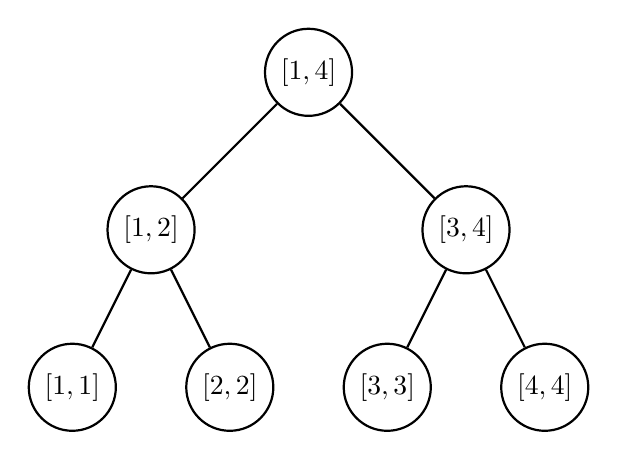
\begin{tikzpicture}
			\node[draw, circle, thick] (1) at (0,4) {$[1, 4]$};

			\node[draw, circle, thick] (2) at (-2,2) {$[1, 2]$};
			\node[draw, circle, thick] (3) at (2,2) {$[3, 4]$};

			\node[draw, circle, thick] (4) at (-3,0) {$[1, 1]$};
			\node[draw, circle, thick] (5) at (-1,0) {$[2, 2]$};
			\node[draw, circle, thick] (6) at (1,0) {$[3, 3]$};
			\node[draw, circle, thick] (7) at (3,0) {$[4, 4]$};

			\path[draw, thick] (1) -- (2);
			\path[draw, thick] (1) -- (3);
			\path[draw, thick] (2) -- (4);
			\path[draw, thick] (2) -- (5);
			\path[draw, thick] (3) -- (6);
			\path[draw, thick] (3) -- (7);
        \end{tikzpicture}
    \end{center}
\end{frame}

\begin{frame}[plain]{Drawn Segment Tree, $n = 7$}
	\begin{center}
		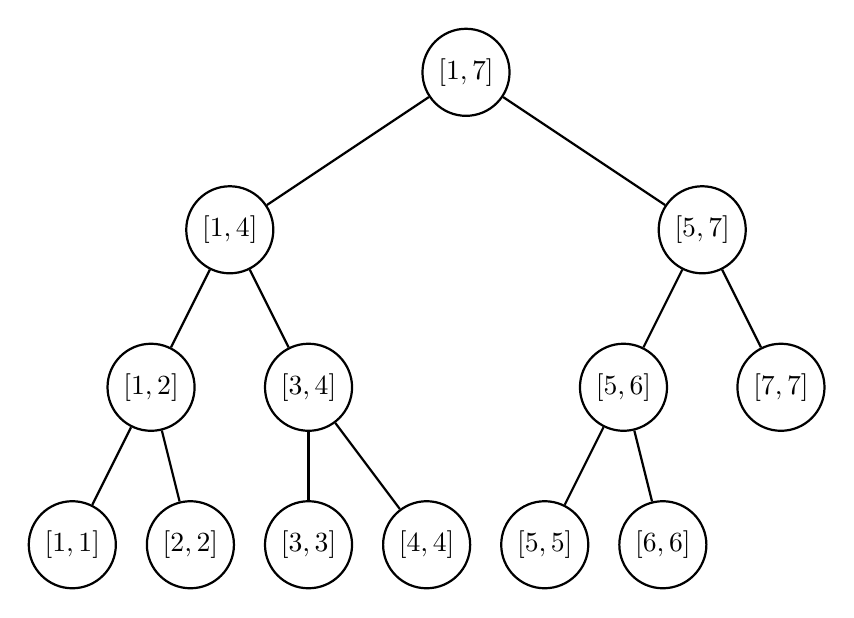
\begin{tikzpicture}
			\node[draw, circle, thick] (1) at (0,6) {$[1, 7]$};

			\node[draw, circle, thick] (2) at (-3,4) {$[1, 4]$};
			\node[draw, circle, thick] (3) at (3,4) {$[5, 7]$};

			\node[draw, circle, thick] (4) at (-4,2) {$[1, 2]$};
			\node[draw, circle, thick] (5) at (-2,2) {$[3, 4]$};
			\node[draw, circle, thick] (6) at (2,2) {$[5, 6]$};
			\node[draw, circle, thick] (7) at (4,2) {$[7, 7]$};

			\node[draw, circle, thick] (8) at (-5,0) {$[1, 1]$};
			\node[draw, circle, thick] (9) at (-3.5,0) {$[2, 2]$};
			\node[draw, circle, thick] (10) at (-2,0) {$[3, 3]$};
			\node[draw, circle, thick] (11) at (-0.5,0) {$[4, 4]$};
			\node[draw, circle, thick] (12) at (1,0) {$[5, 5]$};
			\node[draw, circle, thick] (13) at (2.5,0) {$[6, 6]$};

			\path[draw, thick] (1) -- (2);
			\path[draw, thick] (1) -- (3);
			\path[draw, thick] (2) -- (4);
			\path[draw, thick] (2) -- (5);
			\path[draw, thick] (3) -- (6);
			\path[draw, thick] (3) -- (7);
			\path[draw, thick] (4) -- (8);
			\path[draw, thick] (4) -- (9);
			\path[draw, thick] (5) -- (10);
			\path[draw, thick] (5) -- (11);
			\path[draw, thick] (6) -- (12);
			\path[draw, thick] (6) -- (13);
        \end{tikzpicture}
    \end{center}
\end{frame}

\begin{frame}[plain,fragile]{Segment Tree - Code}
    \begin{minted}[fontsize=\scriptsize]{cpp}
struct segment_tree {
    segment_tree *left, *right;
    int from, to, value;
    segment_tree(int from, int to)
        : from(from), to(to), left(NULL), right(NULL), value(0) { }
};

segment_tree* build(const vector<int> &arr, int l, int r) {
    if (l > r) return NULL;
    segment_tree *res = new segment_tree(l, r);
    if (l == r) {
        res->value = arr[l];
    } else {
        int m = (l + r) / 2;
        res->left = build(arr, l, m);
        res->right = build(arr, m + 1, r);
        if (res->left != NULL) res->value += res->left->value;
        if (res->right != NULL) res->value += res->right->value;
    }
    return res;
}
    \end{minted}
\end{frame}

\begin{frame}[plain]{Updates}
	\begin{center}
		\begin{tikzpicture}
			\only<all:1-2, 14-15, 24-> { \node[draw, circle, thick] (1) at (0,6) {\phantom{xxx}}; }
			\only<all:3-13, 16-23> { \node[draw, circle, thick, red] (1) at (0,6) {\phantom{xxx}}; }


			\only<all:1-3, 12-> { \node[draw, circle, thick] (2) at (-3,4) {\phantom{xxx}}; }
			\only<all:4-11> { \node[draw, circle, thick, red] (2) at (-3,4) {\phantom{xxx}}; }

			\only<all:1-16, 22-> { \node[draw, circle, thick] (3) at (3,4) {\phantom{xxx}}; }
			\only<all:17-21> { \node[draw, circle, thick, red] (3) at (3,4) {\phantom{xxx}}; }


			\only<all:1-> { \node[draw, circle, thick] (4) at (-4,2) {\phantom{xxx}}; }

			\only<all:1-4, 10-> { \node[draw, circle, thick] (5) at (-2,2) {\phantom{xxx}}; }
			\only<all:5-9> { \node[draw, circle, thick, red] (5) at (-2,2) {\phantom{xxx}}; }

			\only<all:1-> { \node[draw, circle, thick] (6) at (2,2) {\phantom{xxx}}; }

			\only<all:1-17, 20-> { \node[draw, circle, thick] (7) at (4,2) {\phantom{xxx}}; }
			\only<all:18-19> { \node[draw, circle, thick, red] (7) at (4,2) {\phantom{xxx}}; }


			\only<all:1-> { \node[draw, circle, thick] (8) at (-5,0) {\phantom{xxx}}; }

			\only<all:1-> { \node[draw, circle, thick] (9) at (-3.5,0) {\phantom{xxx}}; }

			\only<all:1-> { \node[draw, circle, thick] (10) at (-2,0) {\phantom{xxx}}; }

			\only<all:1-5, 8-> { \node[draw, circle, thick] (11) at (-0.5,0) {\phantom{xxx}}; }
			\only<all:6-7> { \node[draw, circle, thick, red] (11) at (-0.5,0) {\phantom{xxx}}; }

			\only<all:1-> { \node[draw, circle, thick] (12) at (1,0) {\phantom{xxx}}; }

			\only<all:1-> { \node[draw, circle, thick] (13) at (2.5,0) {\phantom{xxx}}; }

			\path[draw, thick] (1) -- (2);
			\path[draw, thick] (1) -- (3);
			\path[draw, thick] (2) -- (4);
			\path[draw, thick] (2) -- (5);
			\path[draw, thick] (3) -- (6);
			\path[draw, thick] (3) -- (7);
			\path[draw, thick] (4) -- (8);
			\path[draw, thick] (4) -- (9);
			\path[draw, thick] (5) -- (10);
			\path[draw, thick] (5) -- (11);
			\path[draw, thick] (6) -- (12);
			\path[draw, thick] (6) -- (13);


			\only<all:2-14> { \node at (-3,6) {\texttt{update(3, 7)}}; }
			\only<all:15-24> { \node at (-3,6) {\texttt{update(6, -12)}}; }
			\only<all:25-> { \node at (-3,6) {}; }

			\only<all:1-12> { \node at (0,6) {$40$}; }
			\only<all:13-22> { \node at (0,6) {$47$}; }
			\only<all:23-> { \node at (0,6) {$35$}; }

			\only<all:1-10> { \node at (-3,4) {$16$}; }
			\only<all:11-> { \node at (-3,4) {$23$}; }

			\only<all:1-20> { \node at (3,4) {$24$}; }
			\only<all:21-> { \node at (3,4) {$12$}; }

			\only<all:1-> { \node at (-4,2) {$5$}; }

			\only<all:1-8> { \node at (-2,2) {$11$}; }
			\only<all:9-> { \node at (-2,2) {$18$}; }

			\only<all:1-> { \node at (2,2) {$17$}; }

			\only<all:1-18> { \node at (4,2) {$7$}; }
			\only<all:19-> { \node at (4,2) {$-5$}; }

			\only<all:1-> { \node at (-5,0) {$3$}; }

			\only<all:1-> { \node at (-3.5,0) {$2$}; }

			\only<all:1-> { \node at (-2,0) {$9$}; }

			\only<all:1-6> { \node at (-0.5,0) {$2$}; }
			\only<all:7-> { \node at (-0.5,0) {$9$}; }

			\only<all:1-> { \node at (1,0) {$9$}; }

			\only<all:1-> { \node at (2.5,0) {$8$}; }
        \end{tikzpicture}
    \end{center}
\end{frame}

\begin{frame}[plain,fragile]{Updating a Segment Tree - Code}
    \vspace{40pt}
    \begin{minted}[fontsize=\scriptsize]{cpp}
int update(segment_tree *tree, int i, int val) {
    if (tree == NULL) return 0;
    if (tree->to < i) return tree->value;
    if (i < tree->from) return tree->value;
    if (tree->from == tree->to && tree->from == i) {
        tree->value = val;
    } else {
        tree->value = update(tree->left, i, val) + update(tree->right, i, val);
    }
    return tree->value;
}
    \end{minted}
\end{frame}

\begin{frame}[plain]{Querying}
	\begin{center}
		\begin{tikzpicture}
			\only<all:2-9> { \node at (-3,6) {\texttt{query(1, 7)}}; }
			\only<all:10-17> { \node at (-3,6) {\texttt{query(1, 2)}}; }

			\only<all:8> { \node at (-3,5.5) {\texttt{= 2 + 18 + 12}}; }
			\only<all:9> { \node at (-3,5.5) {\texttt{= 32}}; }
			\only<all:16> { \node at (-3,5.5) {\texttt{= 2 + 9}}; }
			\only<all:17> { \node at (-3,5.5) {\texttt{= 11}}; }



			\only<all:1-2, 4-10, 12-> { \node[draw, circle, thick] (1) at (0,6) {\phantom{xxx}}; }
			\only<all:3, 11> { \node[draw, circle, thick, red] (1) at (0,6) {\phantom{xxx}}; }


			\only<all:1-3, 5-11, 13-> { \node[draw, circle, thick] (2) at (-3,4) {\phantom{xxx}}; }
			\only<all:4, 12> { \node[draw, circle, thick, red] (2) at (-3,4) {\phantom{xxx}}; }

			\only<all:1-3, 10-> { \node[draw, circle, thick] (3) at (3,4) {\phantom{xxx}}; }
			\only<all:4> { \node[draw, circle, thick, red] (3) at (3,4) {\phantom{xxx}}; }
			\only<all:5-9> { \node[draw, circle, thick, blue] (3) at (3,4) {\phantom{xxx}}; }


			\only<all:1-4, 6-12, 14-> { \node[draw, circle, thick] (4) at (-4,2) {\phantom{xxx}}; }
			\only<all:5, 13> { \node[draw, circle, thick, red] (4) at (-4,2) {\phantom{xxx}}; }

			\only<all:1-4, 10-12, 14-> { \node[draw, circle, thick] (5) at (-2,2) {\phantom{xxx}}; }
			\only<all:5, 13> { \node[draw, circle, thick, red] (5) at (-2,2) {\phantom{xxx}}; }
			\only<all:6-9> { \node[draw, circle, thick, blue] (5) at (-2,2) {\phantom{xxx}}; }

			\only<all:1-> { \node[draw, circle, thick] (6) at (2,2) {\phantom{xxx}}; }

			\only<all:1-> { \node[draw, circle, thick] (7) at (4,2) {\phantom{xxx}}; }


			\only<all:1-> { \node[draw, circle, thick] (8) at (-5,0) {\phantom{xxx}}; }

			\only<all:1-5, 10-13, 18-> { \node[draw, circle, thick] (9) at (-3.5,0) {\phantom{xxx}}; }
			\only<all:6, 14> { \node[draw, circle, thick, red] (9) at (-3.5,0) {\phantom{xxx}}; }
			\only<all:7-9, 15-17> { \node[draw, circle, thick, blue] (9) at (-3.5,0) {\phantom{xxx}}; }

			\only<all:1-13, 18-> { \node[draw, circle, thick] (10) at (-2,0) {\phantom{xxx}}; }
			\only<all:14> { \node[draw, circle, thick, red] (10) at (-2,0) {\phantom{xxx}}; }
			\only<all:15-17> { \node[draw, circle, thick, blue] (10) at (-2,0) {\phantom{xxx}}; }

			\only<all:1-> { \node[draw, circle, thick] (11) at (-0.5,0) {\phantom{xxx}}; }

			\only<all:1-> { \node[draw, circle, thick] (12) at (1,0) {\phantom{xxx}}; }

			\only<all:1-> { \node[draw, circle, thick] (13) at (2.5,0) {\phantom{xxx}}; }

			\path[draw, thick] (1) -- (2);
			\path[draw, thick] (1) -- (3);
			\path[draw, thick] (2) -- (4);
			\path[draw, thick] (2) -- (5);
			\path[draw, thick] (3) -- (6);
			\path[draw, thick] (3) -- (7);
			\path[draw, thick] (4) -- (8);
			\path[draw, thick] (4) -- (9);
			\path[draw, thick] (5) -- (10);
			\path[draw, thick] (5) -- (11);
			\path[draw, thick] (6) -- (12);
			\path[draw, thick] (6) -- (13);

			\node at (0,6) {$35$};
			\node at (-3,4) {$23$};
			\node at (3,4) {$12$};
			\node at (-4,2) {$5$};
			\node at (-2,2) {$18$};
			\node at (2,2) {$17$};
			\node at (4,2) {$-5$};
			\node at (-5,0) {$3$};
			\node at (-3.5,0) {$2$};
			\node at (-2,0) {$9$};
			\node at (-0.5,0) {$9$};
			\node at (1,0) {$9$};
			\node at (2.5,0) {$8$};
        \end{tikzpicture}
    \end{center}
\end{frame}


\begin{frame}[plain,fragile]{Querying a Segment Tree - Code}
    \vspace{50pt}
    \begin{minted}[fontsize=\scriptsize]{cpp}
int query(segment_tree *tree, int l, int r) {
    if (tree == NULL) return 0;
    if (l <= tree->from && tree->to <= r) return tree->value;
    if (tree->to < l) return 0;
    if (r < tree->from) return 0;
    return query(tree->left, l, r) + query(tree->right, l, r);
}
    \end{minted}
\end{frame}

\begin{frame}[plain]{Segment Tree}
    \begin{itemize}
        \item<1-> Simple to use Segment Trees for $\min$, $\max$, $\gcd$, and other similar operators, basically the same code.
        \item<2-> Any associative operator will work.
        \item<3-> So any operator $f$ such that $f(a, f(b, c)) = f(f(a, b), c)$ for all $a, b, c$.
        \item<4-> Also possible to update a range of values in $O(\log n)$, which will be covered in bonus slides.
    \end{itemize}
\end{frame}

\begin{frame}[plain]{Example problem: Movie Collection}
    \begin{itemize}
        \item https://open.kattis.com/problems/moviecollection
    \end{itemize}
\end{frame}

\begin{frame}[plain]{Another $\log(n)$ idea}
    \begin{itemize}
        \item<1-> What if we tried something more akin to an array.
        \item<2-> Could we store $\log(n)$ amounts of data per element somehow?
        \item<3-> Yes! For each $i$ we can store the sum on the interval $[i, i + 2^j - 1]$ for $\log$ many $j$.
        \item<4-> Then to retrieve a sum from $i$ to $j$ we always take the biggest chunk we can that's stored at $i$, which will always be at least half.
        \item<5-> Then we continue until we reach $j$, moving $i$ along and collecting the results.
        \item<6-> This is what is known as a sparse table.
    \end{itemize}
\end{frame}

\begin{frame}[plain]{Sparse tables}
    \begin{itemize}
        \item<1-> Calculating all of these values takes $\mathcal{O}(n\log(n))$ because we can calculate the values in order of increasing $j$.
        \item<2-> Then when we calculate the sum of $[i, i + 2^j - 1]$ we just combine the earlier results of $[i, i + 2^{j-1} - 1]$ and $[i + 2^{j-1}, i + 2^j - 1]$.
        \item<3-> Querying takes $\mathcal{O}(\log(n))$, however updating is slow and difficult.
        \item<4-> Why would we then ever use this instead of segment trees?
    \end{itemize}
\end{frame}

\begin{frame}[plain]{Binary lifting}
    \begin{itemize}
        \item<1-> The reason might be is that with sparse tables we can do many things that segment trees can not because of how the results are combined.
        \item<2-> Let us consider binary lifting in particular.
        \item<3-> Suppose we have some function $f$ that rearranges the values $\{0, 1, \dots, n - 1\}$ and we get $q$ queries asking what happens to $x$ if we apply $f$ exactly $m$ times to $x$.
        \item<4-> The naïve solution is to calculate it every time, giving a time complexity of $\mathcal{O}(qm\mathcal{O}(f))$.
        \item<5-> How might we use sparse tables to do better?
    \end{itemize}
\end{frame}

\begin{frame}[plain]{Binary lifting ctd.}
    \begin{itemize}
        \item<1-> Let $f^{[y]}(x)$ denote the result of applying $f$ exactly $y$ times to $x$
        \item<2-> For each $i$ we store $f^{[2^j]}(i)$ as a sparse table
        \item<3-> Then we can compute these in increasing order of $j$, calculating $j = 1$ using $f$ itself and then for larger $j$ letting $f^{[2^j]}(x) = f^{[2^{j-1}]}(f^{[2^{j-1}]}(x))$
        \item<4-> Thus we can precompute the table in $\mathcal{O}(n(\mathcal{O}(f) + \log(n)))$ and each query takes $\mathcal{O}(\log(m))$, a much better time complexity
    \end{itemize}
\end{frame}

\begin{frame}[plain]{Sparse table example}
    \begin{center}
        \begin{tikzpicture}[scale=0.75]
            \draw[step=1,black,thin] (0,0) grid (12, 1);
            \node[align=left] at (13.5,0.5) {$j = 0$};
            \node at (0.5,0.5) {$7$};
            \node at (1.5,0.5) {$1$};
            \node at (2.5,0.5) {$6$};
            \node at (3.5,0.5) {$4$};
            \node at (4.5,0.5) {$8$};
            \node at (5.5,0.5) {$0$};
            \node at (6.5,0.5) {$9$};
            \node at (7.5,0.5) {$2$};
            \node at (8.5,0.5) {$2$};
            \node at (9.5,0.5) {$7$};
            \node at (10.5,0.5) {$1$};
            \node at (11.5,0.5) {$6$};

            \only<2-> {
                \draw[step=1,blue,thin] (0,1) grid (12, 2);
                \node[align=left] at (13.5,1.5) {\color{blue} $j = 1$};
            }
            \foreach \x in {3,4,...,13} {
                \only<\x> {
                    \draw[->, blue] ({0.5+\x-3}, 0.75) -- ({0.5+\x-3}, 1.25);
                    \draw[->, blue] ({1.25+\x-3}, 0.75) -- ({0.75+\x-3}, 1.25); 
                }
            }
            \foreach \x [count=\i] in {8, 7, 10, 12, 8, 9, 11, 4, 9, 8, 7, 6} {
                \pgfmathtruncatemacro{\onlyi}{\i+2}
                \only<\onlyi-> {
                    \node at ({-0.5+\i},1.5) {\color{blue} $\x$};
                }
            }

            \only<14> {
                \draw[->, blue] (11.5, 0.75) -- (11.5, 1.25);
            }

            \only<15-> {
                \draw[step=1,dark green,thin] (0,2) grid (12, 3);
                \node[align=left] at (13.5,2.5) {\color{dark green} $j = 2$};
            }
            \foreach \x in {3,4,...,12} {
                \only<15> {
                    \draw[->, dark green] ({0.5+\x-3}, 1.75) -- ({0.5+\x-3}, 2.25);
                    \draw[->, dark green] ({1.25+\x-2}, 1.75) -- ({0.75+\x-3}, 2.25); 
                }
            }
            \only<15> {
                \draw[->, dark green] (11.5, 1.75) -- (11.5, 2.25);
                \draw[->, dark green] (10.5, 1.75) -- (10.5, 2.25);
            }
            \foreach \x [count=\i] in {18, 19, 18, 21, 19, 13, 20, 12, 16, 14, 7, 6} {
                \only<15-> {
                    \node at ({-0.5+\i},2.5) {\color{dark green} $\x$};
                }
            }

            \only<16-> {
                \draw[step=1,dark yellow,thin] (0,3) grid (12, 4);
                \node[align=left] at (13.5,3.5) {\color{dark yellow} $j = 3$};
            }
            \foreach \x in {3,4,...,10} {
                \only<16> {
                    \draw[->, dark yellow] ({0.5+\x-3}, 2.75) -- ({0.5+\x-3}, 3.25);
                    \draw[->, dark yellow] ({1.25+\x}, 2.75) -- ({0.75+\x-3}, 3.25); 
                }
            }
            \only<16> {
                \draw[->, dark yellow] (11.5, 2.75) -- (11.5, 3.25);
                \draw[->, dark yellow] (10.5, 2.75) -- (10.5, 3.25);
                \draw[->, dark yellow] (9.5, 2.75) -- (9.5, 3.25);
                \draw[->, dark yellow] (8.5, 2.75) -- (8.5, 3.25);
            }
            \foreach \x [count=\i] in {37, 32, 38, 33, 35, 27, 27, 18, 16, 14, 7, 6} {
                \only<16-> {
                    \node at ({-0.5+\i},3.5) {\color{dark yellow} $\x$};
                }
            }

            \only<17> {
                \node at (5, 5) {\texttt{query(1, 8) = 19 + 9 + 2}};
                \draw[red, very thick] (1, 2) -- (2, 2) -- (2, 3) -- (1, 3) -- cycle;
                \draw[red, very thick] (5, 1) -- (6, 1) -- (6, 2) -- (5, 2) -- cycle;

                \draw[red, very thick] (1, 0) -- (5, 0) -- (5, 1) -- (1, 1) -- cycle;
                \draw[red, very thick] (5, 0) -- (7, 0) -- (7, 1) -- (5, 1) -- cycle;
                \draw[red, very thick] (7, 0) -- (8, 0) -- (8, 1) -- (7, 1) -- cycle;
            }

            \only<18> {
                \node at (5, 5) {\texttt{query(0, 9) = 37 + 9}};
                \draw[red, very thick] (0, 3) -- (1, 3) -- (1, 4) -- (0, 4) -- cycle;
                \draw[red, very thick] (8, 1) -- (9, 1) -- (9, 2) -- (8, 2) -- cycle;

                \draw[red, very thick] (0, 0) -- (8, 0) -- (8, 1) -- (0, 1) -- cycle;
                \draw[red, very thick] (8, 0) -- (10, 0) -- (10, 1) -- (8, 1) -- cycle;
            }

        \end{tikzpicture}
    \end{center}
\end{frame}

\begin{frame}[plain]{Example problem: Stikl}
    \begin{itemize}
        \item https://open.kattis.com/problems/stikl
    \end{itemize}
\end{frame}

\end{document}
